\documentclass[11pt, oneside]{article} 
\usepackage{geometry}
\geometry{letterpaper} 
\usepackage{graphicx}
	
\usepackage{amssymb}
\usepackage{amsmath}
\usepackage{parskip}
\usepackage{color}
\usepackage{hyperref}

\graphicspath{{/Users/telliott_admin/Tex/png/}}
% \begin{center} 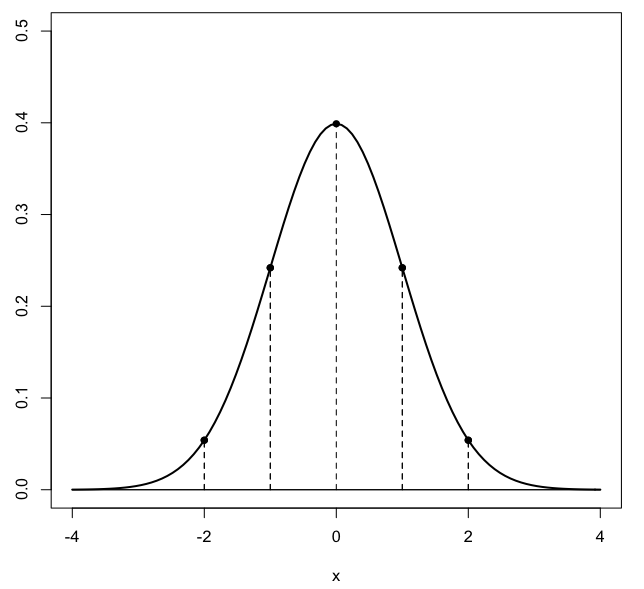
\includegraphics [scale=0.4] {gauss3.png} \end{center}

\title{Gaussian}
\date{}

\begin{document}
\maketitle
\Large

\begin{center} 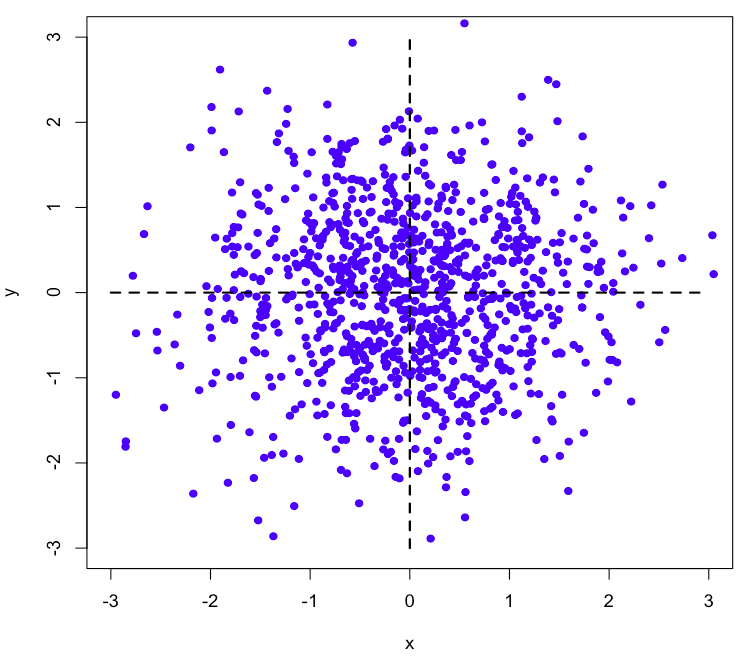
\includegraphics [scale=0.35] {gauss1.png} \end{center}

I'm going show a derivation of the Gaussian distribution from first principles.  The argument is originally due to Sir John F. W. Herschel.

Imagine that you are throwing darts at the origin of the x,y plane. Under perfect conditions, you would hit the center dead on every time. However, conditions aren't perfect. The wind is gusting, the music is loud, there are other distractions. As a result, small errors creep in and the pattern over time looks like the graphic above.

Now, there is some unknown function for the probability that a dart will land in the interval between $x$ and $x + \Delta x$. Obviously, the probability depends on $x$, with a maximum at $x = 0$ and then decreasing to zero as $x$ gets large. We designate that function as a probability density function $p(x)$ and evaluate the density over the interval to get the probability that the dart lands in the interval:

\begin{center} 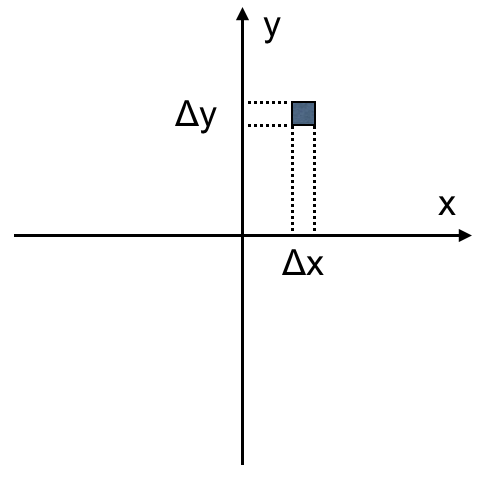
\includegraphics [scale=0.4] {gauss2.png} \end{center}

\[ P = p(x) \Delta x \]
Now we consider a small area of size $\Delta x \Delta y$. If the errors in perpendicular directions are independent, then we expect that we should use the same function $p$ for both $x$ and $y$ and we can get the probability that a dart lands in the small rectangle bounded by $x$, $y$ and $x + \Delta x$, $y + \Delta y$ as:
\[ P = p(x) \Delta x \ p(y) \Delta y\]
In fact, if we assume that the errors do not depend on the orientation of the coordinate system, then the probability is a function only of $r$, the radial distance from the origin, so we can write

\[ P = g(r) \Delta x \ \Delta y \]
\[ g(r) \Delta x \ \Delta y = p(x) \Delta x \ p(y) \Delta y \]
\[ g(r) = p(x)  \ p(y) \]

This assumption of rotational independence leads directly to the answer, as you will see. 

Hamming says, since $r$ does not depend on the angle $\theta$, (but $x$ and $y$ do), we can take the partial derivative with respect to $\theta$ of $g(r)$ and set it equal to zero, so that:

\[ \frac{\partial g(r)}{\partial \theta} = 0 = p(x) \frac{\partial p(y)}{\partial \theta}  + p(y) \frac{\partial p(x)}{\partial \theta} \]

What are these derivatives?
\[ x = r \ cos \theta \]
\[ y = r \ sin \theta \]

\[ \frac{\partial p(x)}{\partial \theta} = \frac{\partial p(x)}{\partial x} \frac{\partial x}{\partial \theta}\]
\[ \frac{\partial x}{\partial \theta} = - r sin \theta \]
\[ \frac{\partial p(x)}{\partial \theta} = p'(x)(-y) \]

\[ \frac{\partial p(y)}{\partial \theta} = \frac{\partial p(y)}{\partial y} \frac{\partial y}{\partial \theta}\]
\[ \frac{\partial y}{\partial \theta} = r cos \theta \]
\[ \frac{\partial p(y)}{\partial \theta} = p'(y)(x) \]
This gives
\[ p(x)p'(y)(x) - p(y)p'(x)(y) = 0 \]
\[ \frac{p'(x)}{p(x)(x)} = \frac{p'(y)}{p(y)(y)} = K \]

What function do we know that has itself as the derivative?

Since 
\[ p'(x) = Kx \ p(x) \]

Clearly, it is exponential, and an exponential with $x^2$
\[ p(x) = A e^{Kx^2/2} \]
\[ p'(x) = AKx \ e^{Kx^2/2} = Kx \ p(x) \]
Since we assume that large errors are less likely than small ones, $K < 0$, so we can define another constant $V = - 1/K$ and
\[ p(x) = A e^{-x^2/2V} \]
This is the normal distribution with variance V.

It is amazing how far we got with this argument! We assumed:
(1) the errors do not depend on the orientation of the coordinate system.
(2) errors in perpendicular directions are independent. This means that being too high doesn't alter the probability of being off to the right.
(3) large errors are less likely than small errors.

Notice that although we started talking about a probability distribution in two dimensions, the function we end up with is for one dimension.

James Clerk Maxwell used the same argument in three dimensions to derive his expression for the distribution of molecular velocities in a gas.

\subsection*{Derivatives}

\begin{center}
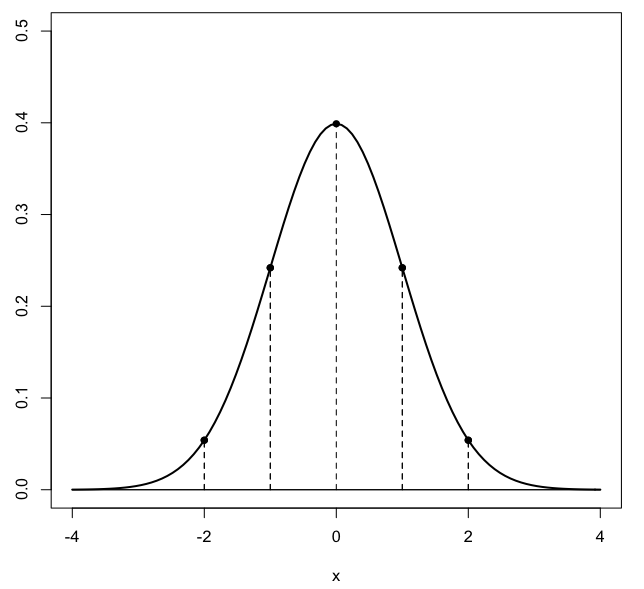
\includegraphics [scale=0.4] {gauss3.png}
\end{center}
The normal or Gaussian distribution, plotted above, is usually divided into sections according to $x = \pm n$ standard deviations.  It's an interesting fact that the first standard deviation corresponds to the inflection point of the curve.  At that point the second derivative of the function is equal to zero.

\[ G(x) = \frac{1}{\sigma \sqrt{2 \pi}} \ exp \ \{ \ -\frac{1}{2} (\frac{x - \mu}{\sigma} )^2\ \} \]
Let
\[ v(x) = -\frac{1}{2} (\frac{x - \mu}{\sigma} )^2 \]
\[ k = \sigma \sqrt{2 \pi} \]
\[ G(x) = \frac{1}{k} \ e^v \]

\[ G'(x) = \frac{1}{k} \  v' e^v\]
\[ \frac{dv}{dx} = -\frac{1}{\sigma} (\frac{x - \mu}{\sigma}) \]
\[ G'(x) = - \frac{1}{k} \  \frac{1}{\sigma} (\frac{x - \mu}{\sigma}) e^v\]

\[ G''(x) = \frac{1}{k} \ (-\frac{1}{\sigma}) (\frac{x - \mu}{\sigma}) (-\frac{1}{\sigma}) (\frac{x - \mu}{\sigma}) e^v + k (\frac{1}{\sigma}) e^v \]
\[ G''(x) = \frac{1}{k} \ (\frac{1}{\sigma^2}) \ [(\frac{x - \mu}{\sigma})^2 - 1] \ e^v \]
We want
\[ G''(x) = 0 \]
where
\[ e^v = exp \ \{ \ -\frac{1}{2} (\frac{x - \mu}{\sigma} )^2\ \} \]
In the limit as $x \to \pm \infty$, the term above approaches $0$, but those are not the solutions we want.  So we need
\[ (\frac{x - \mu}{\sigma})^2 - 1 = 0 \]
\[ (x-\mu)^2 = \sigma^2 \]
\[ x = \mu \pm \sigma \]
The second derivative required some bookkeeping, but was simple in the end.

What about the constant in front?  It's there to make the sum of the area under the probability distribution, the cumulative distribution function, equal $1$.  There is no way to solve the integral.  There is a way to compute its value over the intervals $[-\infty, \infty]$ and $[0,\infty]$;  alternatively, it can be computed numerically for any interval.

If you do that for $e^v$ as defined above (no leading constant $\frac{1}{k} \ $), you find that the value is $k$.  So this is a "normalizing constant", to make the whole thing equal to $1$.

\end{document}